%%%%%%%%%%%%%%%%%%%%%%%%%%%%%%%%%%%%%%%%%%%%%%%%%%%
%
%  New template code for TAMU Theses and Dissertations starting Fall 2012.  
%  For more info about this template or the 
%  TAMU LaTeX User's Group, see http://www.howdy.me/.
%
%  Author: Wendy Lynn Turner 
%	 Version 1.0 
%  Last updated 8/5/2012
%
%%%%%%%%%%%%%%%%%%%%%%%%%%%%%%%%%%%%%%%%%%%%%%%%%%%
%%%%%%%%%%%%%%%%%%%%%%%%%%%%%%%%%%%%%%%%%%%%%%%%%%%%%%%%%%%%%%%%%%%%%%
%%                           SECTION III
%%%%%%%%%%%%%%%%%%%%%%%%%%%%%%%%%%%%%%%%%%%%%%%%%%%%%%%%%%%%%%%%%%%%%

\chapter{\uppercase{Background}}

\section{Reflection Seismology}

Nowadays, reflection seismology (or seismic reflection) is widely used in the petroleum industry to estimate the properties of the Earth's subsurface from reflected seismic waves and explore geophysics using the principles of seismology. The complete processing flow of this method involves data acquisition, data processing, data interpretation and attributes analysis \cite{seisreflectionwiki}. 

As shown in Figure \ref{seismic_reflection}, data acquisition is performed by using seismic sources such as dynamite or air gun generate to spread out seismic waves, which are reflected back from encountered materials underground and then recorded by the receiving sensors. To get data-scientists-usable 2D/3D seismic dataset, the collected seismic wavelet needs to be pre-processed by data processing methods including deconvolution, common-midpoint (CMP) stacking and migration. After data processing, the seismic events are geometrically re-located in either space or time to the location the event occurred in subsurface and create a complete image of subsurface \cite{seisreflectionwiki}. 

The goal of seismic data interpretation and  attributes analysis is to locate the potential petroleum reservoirs from processed seismic reflections map. It involves deep knowledge of seismic attributes, geophysics, and intensive collaborations between data scientists and geophysicists. This thesis focus on develop a scalable and distributed toolkit to facilitates seismic data attributes analytics.   

\begin{figure}[h]
\centering
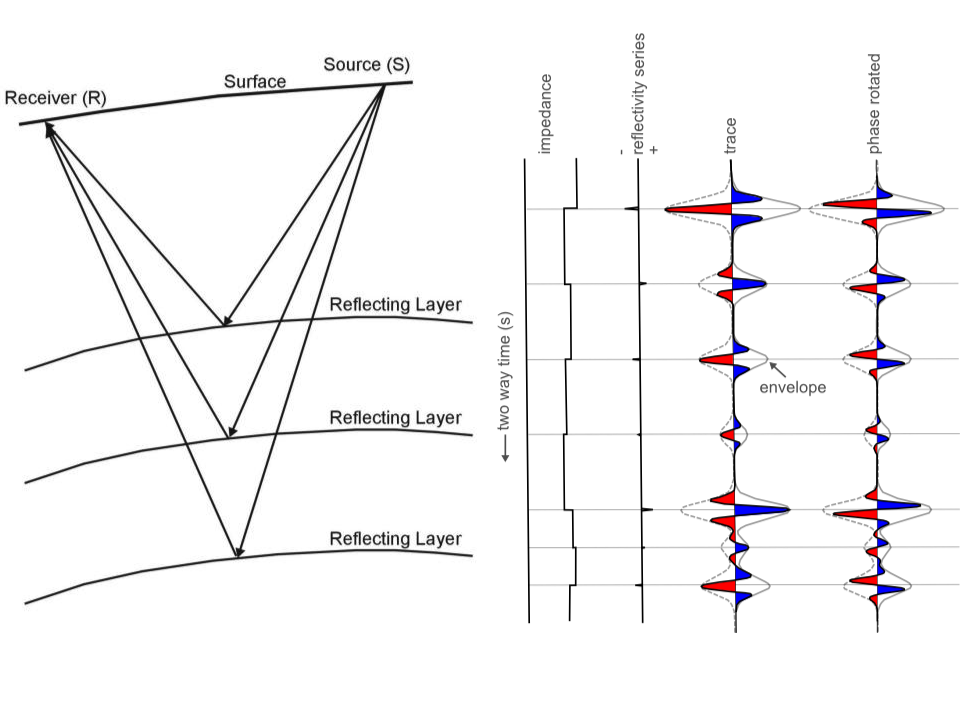
\includegraphics[scale=0.4]{figures/seismic_reflection_principal.png}
\caption{Reflection Seismology \cite{seisreflectionepa} \cite{seisreflectionagile}}
\label{seismic_reflection}
\end{figure}

\section{Big Data Challenge}

The most famous definition of big data, comes from Gartner analyst Doug Laney, specifies the 3Vs characteristics: volume, velocity and variety \cite{demauro2016}. By which volume means the amount of data, velocity stands for the real-time speed of data in and out, and variety is the range of data types and sources. As mentioned in previous section,  the burst increase of volume size, high-speed real-time streaming data from sensors, and various types of structured, unstructured and semi-structured data coming from different stages of seismic data processing all together matches the 3Vs definition. It determines seismic data is costly to store, access and manage in traditional methodology. Therefore, new technology should be adopted to address these problems appropriately.

As the popularity of big data topic grows, there are more and more choices in big data market and open source communities. For instances, Apache Hive and HBase provide the scalable and distributed database solutions,  Apache Storm is capable of handling real-time computation and Apache Kafka is a good choice if users are looking for a distributed streaming platform. These projects provide variety of big data solutions. 

However, all of these big data platforms are designed for general purpose applications and focus on distributing the data, computation and IO overloads. Most MapReduce based framework do not have, or only have limited communication mechanisms between different maps, which is important to resolve the data and logical dependence problems in many complex applications. When it comes to the field of  seismic data processing and analysis, the problem is more complicated. Since most scientists and researchers in petroleum industry do not have big data related knowledge or even computer science background, how to hide parallelism from them and let them easily deploy their works on new platform is a big challenge for all the researchers.

\section{Hadoop File System}

Since Google released its white paper series of big data processing technologies in 2004, the landscape of big data development has been changed profoundly. Many big data projects were inspired and developed based on MapReduce and Google File System framework. Hadoop and Spark is two most widely used open source big data solutions for many business and industry applications in recent years. 

A year after the publication of MapReduce and Google File System framework, Doug Cutting and Mike Cafarella created an open source project Apache Hadoop, which has been utilized in lots of industries to facilitate the works with big volume, variety and velocity of structured and unstructured input datasets \cite{bigdatahistory}. Apache Hadoop consists of Hadoop Distributed File System (HDFS) and MapReduce \cite{ApacheHadoop}.  

Since distributed file system is fundamental to many main stream big data platforms, as it is able to store data across number of storage devices of a cluster, Hadoop Distributed Filesystem becomes one of the most popular Apache subprojects. Originally, HDFS was designed and built for the Apache search engine project Nutch as the file storage infrastructure \cite{ApacheHadoop}. Compare to traditional file system which holds sequential data on one device, HDFS provides far better scalability and support for parallel IO processing mode.

There are some most significant differences that distinguish HDFS from other distributed file systems. First, the high fault-tolerance makes HDFS is able to deployed on low-cost hardware. The high IO throughput access to distributed dataset of HDFS facilitates the applications that have large data sets. Also, HDFS provides streaming access to file system data which is unavailable in conventional POSIX file systems.  

The architecture of a single NameNode and multiple DataNodes in a cluster simplifies the structure of the system. HDFS cluster runs in master-slave mode.  It consists of a single NameNode, the master server which manages the filesystem namespace and the access to distributed datasets, and there are multiple DataNodes, which manage the data storage on the working nodes. HDFS manages the filesystem namespace which enable the general file-form data storage. Files are split into multiple blocks which are saved in multiple DataNodes. The NameNode manages the mapping of data distributions on the DataNodes, and provides general file operations such as open, close, and rename etc. It sends instructions to DataNodes, which perform the related operations on the data blocks and serve the requests of data accessing. Figure \ref{HDFSArch} shows the NameNode-DataNodes architecture of Apache Hadoop File System.

\begin{figure}[h]
\centering
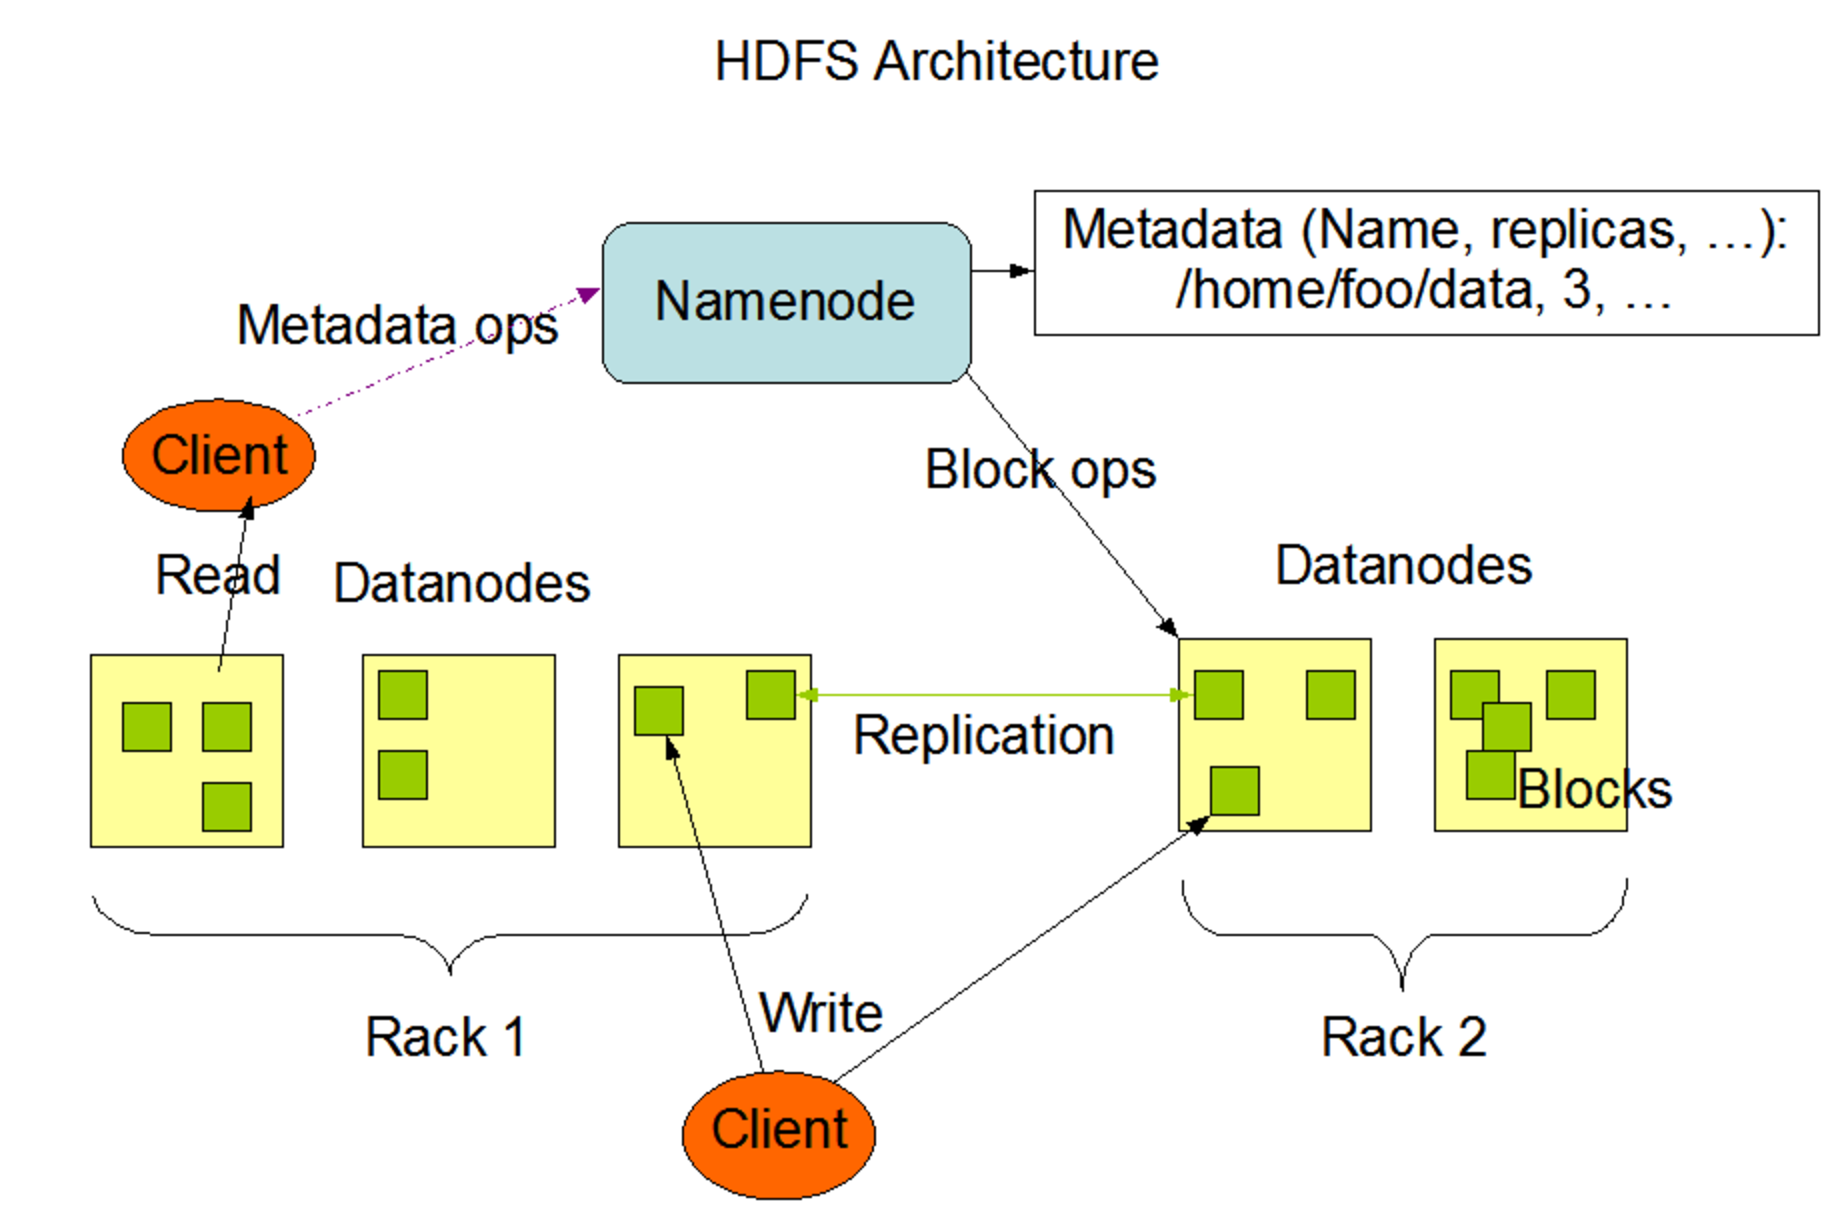
\includegraphics[scale=0.4]{figures/HDFSArch.png}
\caption{The Architecture of Hadoop File System \cite{ApacheHadoop}}
\label{HDFSArch}
\end{figure}

\section{Spark}

The open source big data project Apache Spark provides programmers with an application programming interface centered on a data structure called the resilient distributed dataset (RDD), a fault-tolerant collection of elements that can be operated on in parallel \cite{ApacheSpark}. Since Spark itself does not provide distributed file system, it is usually installed on top of Hadoop, by which Spark could utilize HDFS interface to handle distributed data storage and access. 

The most different part between Hadoop and Spark is the parallel processing interface. MapReduce writes the result back to the storage after each reduction, while Spark utilizes RDD to handle most its operations and result in memory. This leads to up to100 times performance improvement compare to Hadoop in certain circumstances \cite{ApacheSpark}. Another advantage of Spark is it provides more advanced features such as real-time streaming processing interface and machine-learning library.

\subsection{Resilient Distributed Dataset}

Resilient Distributed Dataset (RDD) is distributed data collection with high fault-tolerance and can be accessed and operated in parallel. A RDD can be generated in two way, transforming an existed RDD to a new RDD, or importing the data stored in file storage system. Although Spark supports data loading from both traditional and distributed file system, it is designed for performing on the latter one for the high performance and parallelism. Spark supports any data source providing the Hadoop input format, such as HDFS and HBase \cite{ApacheSpark}.




\subsection{Programming Model}


%%%%%%%%%%%%%%%%%%%%%%%%%%%%%%%%%%%%%%%%%%%%%%%%%%%%%%%
%\subsection{Subsection}

%A table example is going to follow.

%\begin{table}[H]
%\centering
%\caption{This is a table template}
%\begin{tabular}{|l|c|c|c|c|c|}
%\hline
%Product & 1 & 2 & 3 & 4 & 5\\
%\hline
%Price & 124.- & 136.- & 85.- & 156.- & 23.-\\
%Guarantee [years] & 1 & 2 & - & 3 & 1\\
%Rating & 89\% & 84\% & 51\% & & 45\%\\
%\hline
%\hline
%Recommended & yes & yes & no & no & no\\
%\hline
%\end{tabular}
%\label{tab:template2}
%\end{table}
%\subsubsection{This is a subsubsection}


